\chapter{Testing}
\label{chap:case-study}

The thesis now focusses on the application of the implemented features and methods in a real-world scenario. The goal is to demonstrate the practical applicability of the developed concepts and to validate the theoretical findings presented in the previous chapters.

\section{Application Scenario}
\label{sec:factory}
The framework has been applied on the Internet of Things-Factory (IOT) in Gütersloh, Germany \parencite{IoTFactory2024}. It is a cyber-physical system (CPS) \parencite{baheti2011cyber} mimicking industry-relevant processes in a smaller scale for research students. It consists of several stations that are partly interconnected via an assembly line or a delivery service conducted by automatic guided vehicles (AGVs). The factory is modular, so processes can be discovered module-wise in isolation. All modules are working on edge but are connected to a cluster to control it. The factory works without any personnel in theory. The main process also evaluated here is circular, meaning that the product is assembled and can be disassembled in a loop. The factory is shown in Figure \ref{fig:iotoverview}.

\begin{figure}[htbp]
  \centering
  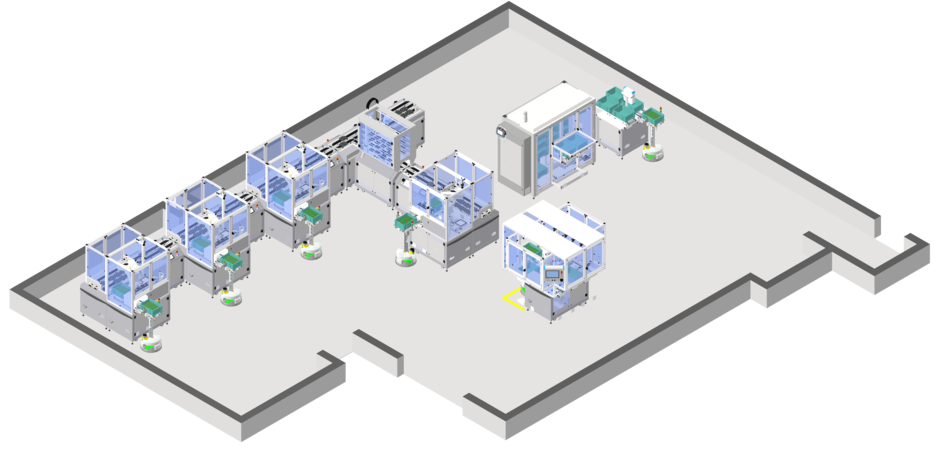
\includegraphics[width=0.7\textwidth]{figures/iot1.png}
  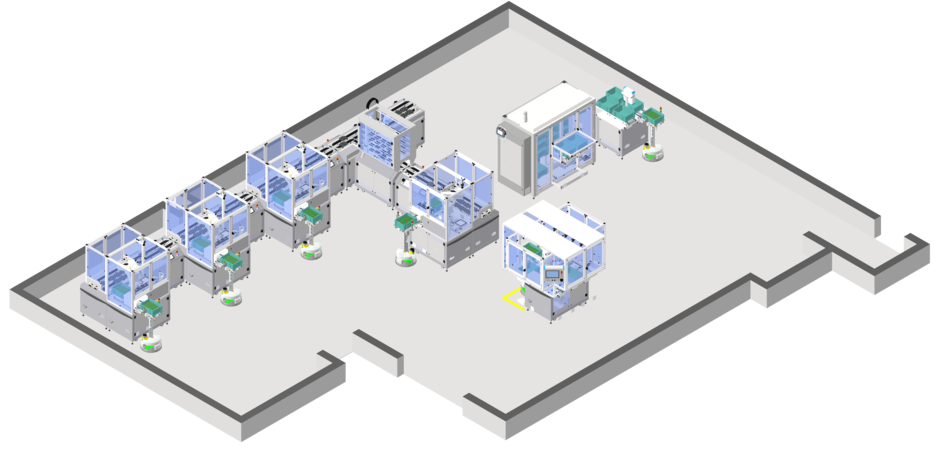
\includegraphics[width=0.7\textwidth]{figures/iot1.png}
  \caption{Overview of the IOT factory. It consists of three production stations from left to right, which are followed by a sorting station and a packaging station. The stations are interconnected by an assembly line. Isolated from the assembly part, two AGVs are used to transport parts between the warehouse station (upper right) and another flexible workstation (right).}
  \label{fig:iotoverview}
\end{figure}

The robot cells are responsible for performing transformation operation like assembling additional parts or testing functions.

\begin{figure}[htbp]
  \centering
  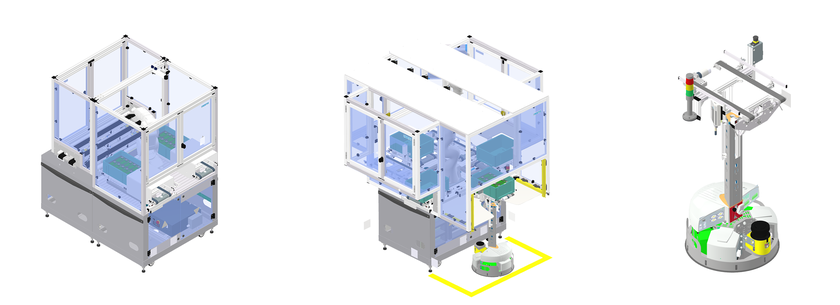
\includegraphics[width=0.8\textwidth]{figures/robots.png}
  \caption{Two robot cells. The first cell is the main actor in this exemplary production process. Cell two is not part of the observed process here. The third image shows an AGV which transports boxes with assembled and disassembled parts to the stations.}
  \label{fig:robots}
\end{figure}

The factory produces an exemplary product, consisting of a back part, a breadboard for several parts and a front panel. The parts to put on the breadboard are a display, gyroscope, an analog board and a weather station.

\begin{figure}[htbp]
  \centering
  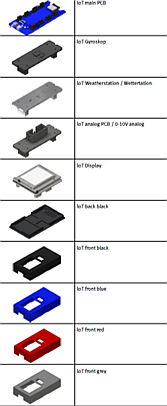
\includegraphics[width=0.2\textwidth]{figures/parts.png}
  \caption{The product consists of a back part, a breadboard and a front panel. The breadboard is used to put on several parts, such as a display, gyroscope, analog board and a weather station.}
  \label{fig:iotproduct}
\end{figure}

The only colour produced at the moment is black. Not all parts can be put on the breadboard and there are several parts which conflict in size and location on the breadboard. The ground-truth assembly rules look as follows:
PRÜFEN UND ANPASSEN

\begin{figure}[htbp]
  \centering
  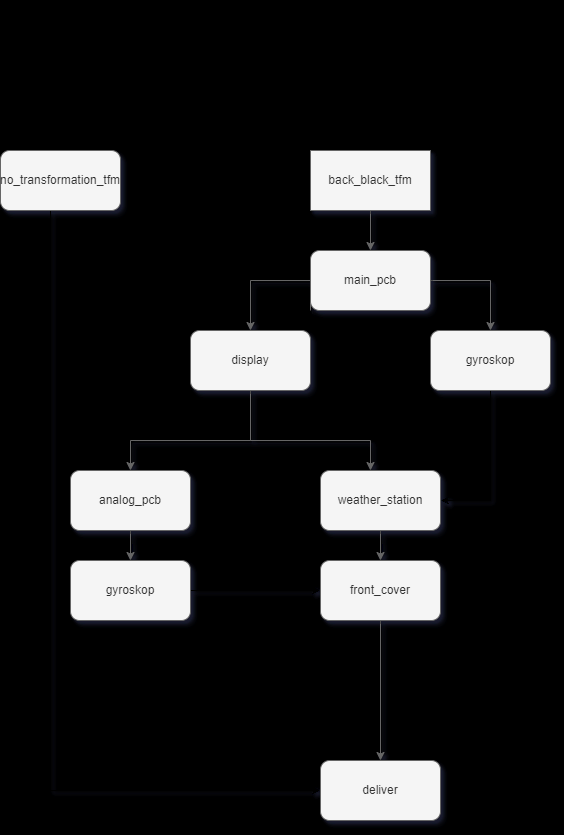
\includegraphics[width=0.8\textwidth]{figures/assrules.png}
  \caption{Three variants are possible. No transformation is also a possibility.}
  \label{fig:assrules}
\end{figure}

Back and front cover are necessary parts and are assembled every time. The main part \texttt{main\_pcb} is also obligatory. It is placed at the beginning. Following that, the display or gyroscope can be assembled. If the display has been chosen, only the analog board or the weather station can be assembled. The weather station takes too much space on the breadboard for the gyroscope to be placed. If the analog board has been placed, the gyroscope is of course possible. The product is finished by placing the front cover and delivering the product to the sink.

During the production, the factory gathers data via sensors. The data is saved in a database and can be used for further analysis.

Finally, the sequential order of the production process is as follows:

\begin{figure}[H]
  \centering
  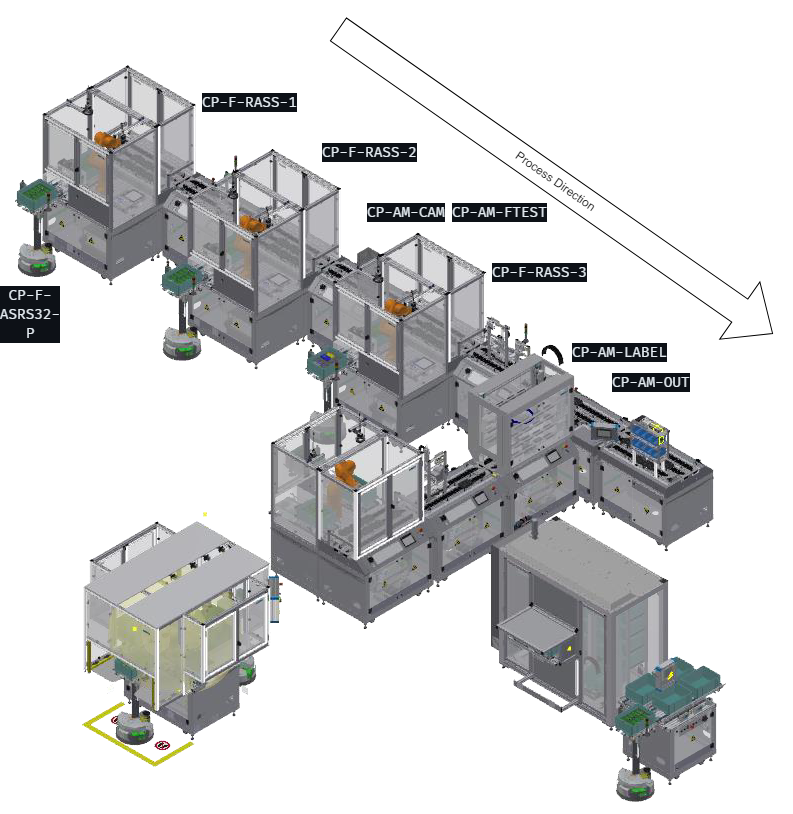
\includegraphics[width=0.7\textwidth]{figures/processdirection.png}
  \caption{The blueprint with transitions between resources.}
  \label{fig:transitions}
\end{figure}

\subsection{Data Basis}

\subsubsection{SBDT Dataset}

The dataset gathered from the SBDT is referred to as \texttt{sim\_data}. The OpenFactoryTwin (see \autoref{sec:automated-digital-twin}) provides a method to deserialize the simulated orders and save them in a CSV file. The dataset then gets converted to the OCEL structure. For this endeveur, a separate connector logic has to be implemented in every use case. See \texttt{src/connector/ofact} for the connector here.

The connector's output follows a standardized structure defined by the \texttt{OutputStructure} class, which ensures consistency across different data sources. The connector first deserializes the dynamic state model from a pickle file, accessing the full simulation state. Only actual process executions (as opposed to planned ones) are retained for further processing, identified by the "ACTUAL" flag in their event type. The connector creates mapping dictionaries for various categorical attributes following the OCED standard:

\begin{itemize}
  \item \textbf{Part ID Mapping:} Uses domain expertise to identify part types from process names, normalizing text (lowercase, no whitespace) to match against a predefined list of possible parts. This list contains possible parts from \autoref{fig:iotproduct}.
  \item \textbf{Process Type Categorization:} Assigns process steps to expert-defined categories such as "machine," "feature," "endproduct," "test," and "transport" based on keywords in process names. These types have been assigned by the modeller and are of free choice. See \autoref{tab:output-structure-detailed}.
  \item \textbf{Process ID Mapping:} Creates unique integer identifiers for each distinct process description based on enumeration.
  \item \textbf{Resource ID Mapping:} Generates unique identifiers for each resource involved in the process executions based on enumeration.
  \item \textbf{Temporal Data Extraction:} The connector extracts start and end times for each process execution.
\end{itemize}

Process executions are associated with their respective order IDs, establishing the connection between individual process steps and the orders they belong to. All extracted information is then consolidated into a standardized DataFrame structure with properly typed columns as defined in the \texttt{OutputStructure} class. The connector also includes a validation step to ensure that the generated DataFrame adheres to the expected structure and data types, raising an error if any discrepancies are found.

A key aspect of the connector's functionality is the integration of domain knowledge into the data transformation process. Instead of relying solely on the raw data structure, the connector employs expert-defined categorizations and normalization procedures to ensure semantic consistency in the transformed data.

For example, the part identification logic uses a predefined list of potential parts (such as "GYROSCOPE," "MAIN PCB," "FRONT COVER," etc.) and searches for these terms within process descriptions. Similarly, the process type categorization uses domain-specific groupings like "machine," "feature," and "test" based on keywords found in process names.This domain knowledge integration ensures that the transformed data maintains the semantic richness required for meaningful validation and comparison between simulated and real-world processes.

The \texttt{sim\_data} rows will receive the label $0$ for \texttt{is\_valid}, because we want the black-box model to learn to distinguish between real and simulated data to perform VVUQ. This way we can ensure that the SBDT learned important characteristics from the factory data, which receives the integer $1$ for \texttt{is\_valid}.

\subsubsection{Factory Dataset}

The dataset has been gathered from the database of the IoT Factory. In the code it is referred to as \texttt{real\_data}.

The dataset contains 18057 rows and 4696 orders from a timespan of 22.04.2020 to 14.05.2024. There are no duplicate rows. Each row describes a unique operation step in an order. Roughly 40 percent of the rows contain missing values, which have been filled with zeros.
The data has been mined from a MariaDB SQL database of the IoT Factory. Several tables have been aggregated to form the dataset. Without additional tables, no information about workplans, resources and operation numbers would be available. The dataset is filtered for promising trajectories of meaningful and intact process executions. The filter considers data between the 20.04.2020 and 22.04.2022, 02.05.2022 and 19.07.2022, 02.11.2022, 11.11.2022, 23.01.2022 and March 2023, each data inclusively.

The dataset contains the following columns:

\begin{itemize}
  \item \textbf{WPNo}: The workplan number of the specific workplan.
  \item \textbf{StepNo}: The step number of the specific workplan. The workplan is divided in sequential steps enumerated by this number.
  \item \textbf{ONo}: The order number of the specific order. Each order has a unique number.
  \item \textbf{OPos}: The order position of the specific order. The order position is the position of the order in the workplan.
  \item \textbf{Description}: The description of the specific step in spoken language.
  \item \textbf{OpNo}: The operation number of the specific operation. Each operation has a unique number.
  \item \textbf{NextStepNo}: The next step number of the specific step. This is the step that follows the current step.
  \item \textbf{FirstStep}: The first step of the specific workplan.
  \item \textbf{ErrorStepNo}: The error step number of the specific step. This is the step that is executed in case of an error.
  \item \textbf{Start}: The start time of the specific step.
  \item \textbf{End}: The end time of the specific step.
  \item \textbf{OPNoType}: The operation number type of the specific operation.
  \item \textbf{ResourceID}: The resource ID of the specific resource.
  \item \textbf{ErrorStep}: Is this step an error step (yes/no)?
  \item \textbf{ErrorRetVal}: The error return value of the specific step.
  \item \textbf{Active}: Is this step active (yes/no)?
  \item \textbf{op\_desc}: The operation description of the specific operation. More specific than the description.
  \item \textbf{ResourceName}: The name of the specific resource.
  \item \textbf{resource\_desc}: The description of the specific resource.
  \item \textbf{workplan\_desc}: The description of the specific workplan.
  \item \textbf{workplantype\_desc}: The description of the specific workplan type.
  \item \textbf{case\_id}: The case ID of the specific case.
  \item \textbf{Description\_Encoded}: The description of the specific step ordinally encoded.
\end{itemize}

The operations performed can be seen in the following:

\begin{enumerate}
  \item \textbf{Release a part on stopper 1}: The AGV delivered the box with the parts to be manufactured to the first station. The box is travelling over the assembly line to the first station where the first part is released.
  \item \textbf{Place cover to assembly place}: The first part is placed on the assembly place. The cover is placed on top of the part as the first piece of the product.
  \item \textbf{Assemble part from box on RASS1 - MAIN PCB}: The main PCB is assembled on the cover. This is the first configured part of the product. The main PCB is the breadboard of the product.
  \item \textbf{Switch on PCB}: The main PCB is switched on. This is necessary to activate it.
  \item \textbf{Assemble part from box on RASS1 - DISPLAY}: The display is assembled on the main PCB. This is the second configured part of the product. The display is one optional part of the product. This factors out one product variant.
  \item \textbf{Move part to pallet on belt}: The product is moved to the pallet on the belt for further processing.
  \item \textbf{Measure a part (analog)}: The product is measured. This is necessary to ensure the quality of the product for later steps.
  \item \textbf{Assemble part from box on RASS2 - ANALOG}: The analog part is assembled on the product. This is the third configured part of the product. The analog part is also one optional part of the product.
  \item \textbf{Assemble part from box on RASS2 - GYROSCOPE}: The gyroscope is assembled on the product. This is the fourth configured part of the product. The gyroscope is also one optional part of the product.
  \item \textbf{Move part to pallet on belt}: The product is moved to the pallet on the belt for further processing.
  \item \textbf{Check analog}: The analog part is checked. This is necessary to ensure the quality of the product for later steps.
  \item \textbf{Check gyroscope}: The gyroscope is checked. This is necessary to ensure the quality of the product for later steps
  \item \textbf{Assemble part from box on RASS3 - FRONT COVER}: The front cover is assembled on the product. This is the last configured part of the product. The front cover is the last part of the product.
  \item \textbf{Move part to pallet on belt}: The product is moved to the pallet on the belt for further processing.
  \item \textbf{Test connection to IoT main PCB}: The connection to the IoT main PCB is tested. This is necessary to ensure the quality of the product for later steps.
  \item \textbf{Test the function of the touch display}: The touch display is tested. This is necessary to ensure the quality of the product for later steps.
  \item \textbf{Test the analog input/output shield}: Analog PCB is tested.
  \item \textbf{Test the historical gyroscope data}: The gyroscope is tested.
  \item \textbf{Print Label}: The label is printed. The label contains information about the product configuration, the time manufactured and the serial number.
  \item \textbf{Deliver Part}: The final product is delivered to the sink.
\end{enumerate}

Per step, several resources are involved. The following table shows the utilized resources per step:

\begin{table}[H]
  \centering
  \caption{Steps and Resources Used}
  \label{tab:description-resources}
  \begin{tabular}{@{}p{0.4\textwidth}p{0.4\textwidth}@{}}
    \toprule
    \textbf{Process Step Name}                    & \textbf{Resource Name}                \\
    \midrule
    Release a part on stopper 1                   & CP-F-ASRS32-P                         \\
    Place cover to assembly place                 & CP-F-RASS-1, CP-F-RASS-2, CP-F-RASS-3 \\
    Assemble part from box on RASS1 - MAIN PCB    & CP-F-RASS-1                           \\
    Switch on PCB                                 & CP-F-RASS-1                           \\
    Assemble part from box on RASS1 - DISPLAY     & CP-F-RASS-1                           \\
    Move part to pallet on belt                   & CP-F-RASS-1, CP-F-RASS-2, CP-F-RASS-3 \\
    Measure a part (analog)                       & CP-AM-MEASURE                         \\
    Assemble part from box on RASS2 - ANALOG      & CP-F-RASS-2                           \\
    Assemble part from box on RASS2 - GYROSCOPE   & CP-F-RASS-2                           \\
    Move part to pallet on belt                   & CP-F-RASS-1, CP-F-RASS-2, CP-F-RASS-3 \\
    Check analog                                  & CP-AM-CAM                             \\
    Check gyroscope                               &                                       \\
    Assemble part from box on RASS3 - FRONT COVER & CP-F-RASS-3                           \\
    Move part to pallet on belt                   & CP-F-RASS-1, CP-F-RASS-2, CP-F-RASS-3 \\
    Test connection to IoT main PCB               & CP-AM-FTEST                           \\
    Test the function of the touch display        & CP-AM-FTEST                           \\
    Test the analog input/output shield           & CP-AM-FTEST                           \\
    Test the historical gyroscope data            & CP-AM-FTEST                           \\
    Print Label                                   & CP-AM-LABEL                           \\
    Deliver Part                                  & CP-AM-OUT                             \\
    \bottomrule
  \end{tabular}
\end{table}


This process has been identified as the ground-truth process. The process is circular, meaning that the product is assembled and can be disassembled in a loop. The process is also modular, meaning that the product can be assembled in different configurations. The process is also flexible, meaning that the product can be assembled in different ways.

\section{Open Factory Twin}
\label{sec:automated-digital-twin}

The Simulation-Based Digital Twin (SBDT) for the IoT Factory use case was developed using the Open Factory Twin (OFacT) framework \autocite{ofactintern}. OFacT is an open-source digital twin framework specifically designed for modeling, simulating, and controlling production and logistics environments. Its goal is to support system design, planning, and operational control throughout the entire lifecycle of such systems.

A principle of OFacT is the separation between the static description of the system and its dynamic behavior. This is achieved by distinguishing between:

\begin{itemize}
  \item \textbf{State Model:} This component represents the static structure of the factory, its components (resources, parts, layout), their properties, relationships, and the potential processes or behaviors they can exhibit.
  \item \textbf{Agent Control:} This component implements the dynamic logic that governs the system's operation during simulation, making decisions about resource allocation, process execution sequences, and handling events based on the state model.
\end{itemize}

The construction of the State Model within OFacT uses structured input methods, such as Excel files, where different sheets correspond to specific classes within the OFacT metamodel. To model the IoT Factory scenario (\autoref{sec:factory}), the relevant components of the OFacT State Model were defined, including:

\begin{itemize}
  \item \textbf{Plant}: The overall entity of production. The plant name used here was \texttt{iot\_factory}.
  \item \textbf{EntityType}: All entities have to be defined here. This ranges from the parts, resources and AGVs to the factory itself. For a complete list see the excel document \texttt{small.xlsx} on the second sheet.
  \item \textbf{StationaryResource}: Stationary resources are static and can not move. In this case, these are the RASS stations, measurement-, cam-, function test- and labelling station. The AGVs are not stationary resources, because they can move.
  \item \textbf{Storage}: Storage units contain parts. They are used to traverse the parts through the factory. In this context, the warehouse and box storage, have been modelled.
  \item \textbf{Warehouse}: This is a static storage unit where the parts are stored in boxes until they are processed.
  \item \textbf{WorkStation}: Workstations are resources which perform processes on parts. In our use case, these are the RASS stations.
  \item \textbf{ConveyorBelt}: There is one belt where the storage units traverse through the factory.
  \item \textbf{NonStationaryResource}: There are no non-stationary resources.
  \item \textbf{PassiveMovingResource}: One artifical passive moving resource has been mod
  \item \textbf{Process}: Contains processes and value added processes (VAP). VAP are adding features to parts and modify it. For each activity in the data a VAP has been created.
  \item \textbf{ProcessController}: This controller summarizes all processes to come and connects them.
  \item \textbf{ResourceModel}: Resource groups are formulated for activities like montage, identifying to attach the relevant parts to these resources. This way, main resources and parts are getting matched.
  \item \textbf{ProcessTimeModel}: Each part receives a time simple time distribution to account for its production time.
  \item \textbf{QualityModel}: Each part receives a bernoulli distribution to account for its quality. In the dataset, no quality information existed.
  \item \textbf{TransitionModel}: This model connects possible origins to possible destinations, to that the traversal of the parts can be modelled correctly. The packaging has been modelled as transition model.
  \item \textbf{TransformationModel}: This model contains an artificial transformation model.
  \item \textbf{Time}: Process execution plans get a starting time here.
  \item \textbf{Part}: Parts are connected to their EntityType here. There is also information attached where the part is stored or situated in.
  \item \textbf{Sales}: Lists the features and feature cluster. This matches the building rules. Parts have to be defined as features here.
  \item \textbf{CustomerGeneration}: Customer generation logic.
  \item \textbf{Customer}: List of customers.
  \item \textbf{Orders}: The orders with their requested features.
  \item \textbf{Process}: Contains processes and value added processes (VAP). VAP are adding features to parts and modify it. For each activity in the data a VAP has been created.
  \item \textbf{TransitionModel}: This model connects possible origins to possible destinations, to that the traversal of the parts can be modelled correctly. The packaging has been modelled as transition model.
  \item \textbf{TransformationModel}: This model contains an artificial transformation model.
\end{itemize}


By defining these elements according to the IoT Factory's characteristics, a detailed static model was created within the OFacT framework. For simulation purposes, the state model then gets 'played out' with orders. The orders contain this model then served as the basis for running simulations to generate process execution data, forming the SBDT dataset used in this thesis for comparison against real-world data. The \autoref{fig:assrules} are inherently modelled by the chosen order variants.

\section{Simulation}

The dataset gathered from the SBDT is referred to as \texttt{sim\_data}. The OpenFactoryTwin (see \autoref{sec:automated_digital_twin}) provides a method to deserialize the simulated orders and save them in a CSV file. The dataset then gets converted to the OCEL structure. For this endeveaur, a separate connector logic has to be implemented in every use case. See \texttt{src/connector/ofact} for the connector here.

The connector's output follows a standardized structure defined by the \texttt{OutputStructure} class, which ensures consistency across different data sources. The connector first deserializes the dynamic state model from a pickle file, accessing the full simulation state. Only actual process executions (as opposed to planned ones) are retained for further processing, identified by the "ACTUAL" flag in their event type. The connector creates mapping dictionaries for various categorical attributes following the OCED standard:

\begin{itemize}
  \item \textbf{Part ID Mapping:} Uses domain expertise to identify part types from process names, normalizing text (lowercase, no whitespace) to match against a predefined list of possible parts. This list contains possible parts from \autoref{fig:iotproduct}.
  \item \textbf{Process Type Categorization:} Assigns process steps to expert-defined categories such as "machine," "feature," "endproduct," "test," and "transport" based on keywords in process names. These types have been assigned by the modeller and are of free choice. See \autoref{tab:output-structure-detailed}.
  \item \textbf{Process ID Mapping:} Creates unique integer identifiers for each distinct process description based on enumeration.
  \item \textbf{Resource ID Mapping:} Generates unique identifiers for each resource involved in the process executions based on enumeration.
  \item \textbf{Temporal Data Extraction:} The connector extracts start and end times for each process execution.
\end{itemize}

Process executions are associated with their respective order IDs, establishing the connection between individual process steps and the orders they belong to. All extracted information is then consolidated into a standardized DataFrame structure with properly typed columns as defined in the \texttt{OutputStructure} class. The connector also includes a validation step to ensure that the generated DataFrame adheres to the expected structure and data types, raising an error if any discrepancies are found.

A key aspect of the connector's functionality is the integration of domain knowledge into the data transformation process. Instead of relying solely on the raw data structure, the connector employs expert-defined categorizations and normalization procedures to ensure semantic consistency in the transformed data.

For example, the part identification logic uses a predefined list of potential parts (such as "GYROSCOPE," "MAIN PCB," "FRONT COVER," etc.) and searches for these terms within process descriptions. Similarly, the process type categorization uses domain-specific groupings like "machine" "feature" and "test" based on keywords found in process names.This domain knowledge integration ensures that the transformed data maintains the semantic richness required for meaningful validation and comparison between simulated and real-world processes.

The \texttt{sim\_data} rows will receive the label $0$ for \texttt{is\_valid}, because we want the black-box model to learn to distinguish between real and simulated data to perform VVUQ. This way we can ensure that the SBDT learned important characteristics from the factory data, which receives the integer $1$ for \texttt{is\_valid}.


\subsection{Concatenation of Datasets}

Several preprocessing steps had to be performed to account for the fact that the SBDT simulated only one variant of the product: 'analog', 'cover', 'display', 'gyroscope', 'pcb' and the involved machines. This yielded the necessity to make both datasets congruent to each other. The following steps were performed:

\begin{itemize}
  \item The \texttt{sim\_data} dataset was aligned for the same time period as the \texttt{real\_data} dataset. The SBDT chose the time of order as the production time. In the modelling phase, when adaptive feature selection had been performed to identify if the SBDT was able to learn the Time Model, only \textit{relative} time features were chosen which were developed in \autoref{sec:feature-engineering}.
  \item The \texttt{real\_data} dataset was filtered for the same process steps as the \texttt{sim\_data} dataset. This means that only the process steps which are present in the \texttt{sim\_data} dataset were kept, producing only one product variant. This has also been applied on the part_id, the process_type and resource_id columns. The IDs based on enumeration had to be mapped to the original IDs in \texttt{real\_data} to ensure that the correct IDs are used in the simulation. The mapping was done through the JSON files generated by the connector.
  \item Both datasets have been cleaned and entries containing invalid IDs were removed. This means that all entries which are not present in the mapping dictionaries were removed. The mapping dictionaries are generated by the connector and contain only valid IDs per definition.
  \item Only a subset of all performed processes was included (in detail, all \texttt{process\_id} \le 26. These processes all have the \texttt{process\_type} 'machine', 'feature' or 'endproduct'. The processes with the \texttt{process\_type} 'test' and 'transport' were removed. This was done to ensure that only the relevant processes are included in the dataset.
\end{itemize}

The \texttt{real\_data} dataset was then concatenated with the \texttt{sim\_data} dataset. The concatenation was done by appending the \texttt{sim\_data} dataset to the \texttt{real\_data} dataset. The resulting dataset contains all process steps from both datasets. The resulting dataset is referred to as \texttt{final\_data}. The unification before concatenation was necessary to ensure that no logical flaws are present in the data.

The \texttt{final\_data} dataset finally after preprocessing as described contains 1978 rows and 56 orders with 24 features. The following section elaborates how these features were generated.

\subsubsection{Feature Engineering}


\section{Automatically Generated Digital Twin}
\label{sec:automated-digital-twin}

% Model generation process
% Model properties and parameters
% Aspects of automatic model generation in practice (→ reference to 3.2)
% TODO: Change text
The simulation is conducted using an updated version of the Open Factory Twin (ofact) \parencite{ofact2024}. The dataset was fed in the twin after preprocessing steps were made. For the simulation, the entire time horizon of the dataframe was used and a state model was generated. To achieve this, the IoT factory had to be subsumed under the vocabulary of the twin. The ofact twin has great similarity to the framework by \textcite{Schwede2024}. There are the following aspects in the twin which needed to be filled with information of the factory (see \texttt{small.xlsx} sheets from left to right as well):

\begin{itemize}
  \item \textbf{Plant}: The overall entity of production. The plant name used here was \texttt{iot\_factory}.
  \item \textbf{EntityType}: All entities have to be defined here. This ranges from the parts, resources and AGVs to the factory itself. For a complete list see the excel document \texttt{small.xlsx} on the second sheet.
  \item \textbf{Resource}: Because we model the resources more specifically, we did not use this functionality.
  \item \textbf{StationaryResource}: Stationary resources are static and can not move. In our case, we modelled an artifical obstance to simulate production problems if wanted. This was not relevant here.
  \item \textbf{Storage}: Storage units contain parts. They are used to traverse the parts through the factory. In this context, I modelled the sink, a box and a carrier unit which contains the parts to be assembled.
  \item \textbf{Warehouse}: This is a static storage unit where the parts are stored in boxes until they are processed. In this case, this is the 'Hochregallager' of the factory.
  \item \textbf{WorkStation}: Workstations (or assembly stations in an older version of ofact) are resources which perform processes on parts. In our use case, these are the RASS stations, measurement-, cam-, function test- and labelling station.
  \item \textbf{ConveyorBelt}: There is one belt where the storage units traverse through the factory.
  \item \textbf{NonStationaryResource}: There are no non-stationary resources.
  \item \textbf{ActiveMovingResource}: There are no active moving resources.
  \item \textbf{PassiveMovingResource}: The product carrier, box and sink are modelled as passive moving resources.
  \item \textbf{Process}: Contains processes and value added processes (VAP). VAP are adding features to parts and modify it. There are \(n\) VAP for \(n\) features (like gyroscope, weather station and more). Additional processes for activities like taking a photo of the product through the cam station are also added here.
  \item \textbf{ProcessController}: This controller summarizes all processes to come and connects them.
  \item \textbf{ResourceModel}: Resource groups are formulated for activities like montage, identifying to attach the relevant parts to these resources. This way, main resources and parts are getting matched.
  \item \textbf{ProcessTimeModel}: Each part receives a time simple time distribution to account for its production time.
  \item \textbf{QualityModel}: Each part receives a bernoulli distribution to account for its quality. In the dataset, no quality information existed.
  \item \textbf{TransitionModel}: This model connects possible origins to possible destinations, to that the traversal of the parts can be modelled correctly. Each part and additional processes are relevant here.
  \item \textbf{TransformationModel}: This model contains the building rules from Section \ref{sec:casestudy}.
  \item \textbf{Time}: Process execution plans get a starting time here.
  \item \textbf{Part}: Parts are connected to their EntityType here. There is also information attached where the part is stored or situated in.
  \item \textbf{Sales}: Lists the features and feature cluster. This matches the building rules. Parts have to be defined as features here.
  \item \textbf{CustomerGeneration}: Customer generation logic.
  \item \textbf{Customer}: List of customers.
  \item \textbf{Orders}: The orders with their requested features.
\end{itemize}
\section{VVUQ Experiments}
% Experimental design
% Execution of automated validation
%  model adjustment
% Feature Engineering: Creation of features such as "duration," "sequence_number," and periodic time features (e.g., "day_of_week_sin," "hour_of_day_cos") (→ Reference to 4.3)
% Machine Learning Models: Implementation of a Decision Tree Classifier and an BiLSTM model for validation (→ Reference to 4.3)
% Empirical verification of theoretical V\&V concepts (→ reference to 2.2 and 4.3)


\section{Results and Interpretation}
% Model accuracy and reliability
% xAI
% Analysis of validation metrics (→ Reference to 4.4)
% Discrepancies and Anomalies: Identification of discrepancies between real and simulated data (→ Reference to 7.3)
% Evaluation of results in the context of V\&V theory (→ reference to 2.2)

\section{Comparison with Manual Validation Methods}
% Effort analysis
% Quality comparison
% Cost-benefit analysis
% Empirical evidence for the advantages of automated V\&V (→ reference to 3.2 and 7.3)